%!TeX program = xelatex
\documentclass[10.5pt,hyperref,a4paper,UTF8]{ctexart}
\usepackage{RUCReport}
\usepackage{listings}
\usepackage{xcolor}
\usepackage{threeparttable}
\usepackage{booktabs}
\usepackage{array}
\usepackage{subcaption}
\usepackage{graphicx}
\usepackage{geometry}
\usepackage{float}
\usepackage{tabularx}
\usepackage{booktabs} % 更美观的表格线条
\usepackage{tikz}
\usetikzlibrary{arrows.meta,calc,positioning,decorations.pathreplacing}
\geometry{a4paper, margin=1in}
\renewcommand\thesubfigure{\arabic{subfigure}} % 子图编号改为中文小写
% 定义可能使用到的颜色
\definecolor{CPPLight}  {HTML} {686868}
\definecolor{CPPSteel}  {HTML} {888888}
\definecolor{CPPDark}   {HTML} {262626}
\definecolor{CPPBlue}   {HTML} {4172A3}
\definecolor{CPPGreen}  {HTML} {487818}
\definecolor{CPPBrown}  {HTML} {A07040}
\definecolor{CPPRed}    {HTML} {AD4D3A}
\definecolor{CPPViolet} {HTML} {7040A0}
\definecolor{CPPGray}  {HTML} {B8B8B8}
\definecolor{keywordcolor}{rgb}{0.8,0.1,0.5}
\definecolor{webgreen}{rgb}{0,.5,0}
\definecolor{bgcolor}{rgb}{0.92,0.92,0.92}

\makeatletter
\renewcommand\@cite[2]{\textsuperscript{[#1]}} % 将引用变为右上角的形式
\makeatother

\hypersetup{
    citecolor=black,  % 修改文献引用的颜色为黑色
}

\lstset{
    breaklines = true,                                   % 自动将长的代码行换行排版
    extendedchars=false,                                 % 解决代码跨页时,章节标题,页眉等汉字不显示的问题
    columns=fixed,       
    numbers=left,                                        % 在左侧显示行号
    basicstyle=\zihao{-5}\ttfamily,
    numberstyle=\small,
    frame=none,                                          % 不显示背景边框
    % backgroundcolor=\color[RGB]{245,245,244},            % 设定背景颜色
    keywordstyle=\color[RGB]{40,40,255},                 % 设定关键字颜色
    numberstyle=\footnotesize\color{darkgray},           % 设定行号格式
    commentstyle=\it\color[RGB]{0,96,96},                % 设置代码注释的格式
    stringstyle=\rmfamily\slshape\color[RGB]{128,0,0},   % 设置字符串格式
    showstringspaces=false,                              % 不显示字符串中的空格
    % frame=leftline,topline,rightline, bottomline         %分别对应只在左侧,上方,右侧,下方有竖线
    frame=shadowbox,                                     % 设置阴影
    rulesepcolor=\color{red!20!green!20!blue!20},        % 阴影颜色
    basewidth=0.6em,
}

\lstdefinestyle{CPP}{
    language=c++,                                        % 设置语言
    morekeywords={alignas,continute,friend,register,true,alignof,decltype,goto,
    reinterpret_cast,try,asm,defult,if,return,typedef,auto,delete,inline,short,
    typeid,bool,do,int,signed,typename,break,double,long,sizeof,union,case,
    dynamic_cast,mutable,static,unsigned,catch,else,namespace,static_assert,using,
    char,enum,new,static_cast,virtual,char16_t,char32_t,explict,noexcept,struct,
    void,export,nullptr,switch,volatile,class,extern,operator,template,wchar_t,
    const,false,private,this,while,constexpr,float,protected,thread_local,
    const_cast,for,public,throw,std},
    emph={map,set,multimap,multiset,unordered_map,unordered_set,
    unordered_multiset,unordered_multimap,vector,string,list,deque,
    array,stack,forwared_list,iostream,memory,shared_ptr,unique_ptr,
    random,bitset,ostream,istream,cout,cin,endl,move,default_random_engine,
    uniform_int_distribution,iterator,algorithm,functional,bing,numeric,},
    emphstyle=\color{CPPViolet}, 
}

\lstdefinestyle{Java}{
    language=[AspectJ]Java,
    keywordstyle=\color{keywordcolor}\bfseries
}

\lstdefinestyle{Python}{
    language=Python,
}


%%-------------------------------正文开始---------------------------%%
\begin{document}

%%-----------------------封面--------------------%%
\cover

%%------------------摘要-------------%%
\begin{abstract}
%
XXXXX\\
\textbf{关键词:}XXX
%
\end{abstract}

%%--------------------------目录页------------------------%%
\newpage
\tableofcontents
\thispagestyle{empty} % 目录不显示页码

%%------------------------正文页从这里开始-------------------%
\newpage
\setcounter{page}{1} % 让页码从正文开始编号

%%可选择这里也放一个标题
\begin{center}
    \title{ \Huge \textbf{} }
\end{center}


\thispagestyle{empty} % 首页不显示页码


\section{Interface(API and ADT) vs data structure}
Interface can be called as specification, specify what data can be stored,
whereas the data structure will give an actual representation and tell how to store it.
In the interface, you specify what the operations do, what operations are supported, and in some sense, what they mean.
And the data structure actually gives you algorithms-- this is where the algorithms come in for how to support those operations.

\section{Two main interfaces:set and sequence}
\subsection{static sequence interface}
The number of items doesn't change, though the items might.
\begin{itemize}
    \item size(): return the number of items in the sequence
    \item get(i): return the item at position i
    \item set(i,x): set the item at position i to x
\end{itemize}

\subsection{dynamic sequence interface}
The number of items can change, and the items can be moved around.
\begin{itemize}
    \item insert(i,x): insert x at position i
    \item remove(i): remove the item at position i
\end{itemize}

\subsection{link list}
We store items in a bunch of nodes, each node has an item in it and a next field.
These can be considered as class objects with two class variables, the item and the next pointer.


Insert and delete\_first cost $\theta(1)$ time, but get cost $\theta(n)$ time.
\subsection{static array}
Insert and delete cost $\theta(n)$ time. For 2 reasons, reason 1 is that,
if we are near the front, the we have to do shifting. In a static array, this is not a problem, but in a dynamic array, it can be.
reason 2 is that you are not allowed to change the number of items, so you have to allocate a new array.
you need to copy all the items over, and that takes $\theta(n)$ time.

\subsection{dynamic array(Python lists)}
The idea is to relax the constraint(约束) or the invariant(不变式), 
whatever that the size of the array we use equals n, which is the number
of items in the sequence.
We enforce that the size of the array is $\theta(n)$ \-\- 
probably also greater than or equal to $n$.
We are still going to maintain that the ith item of the array represents $x_i$.

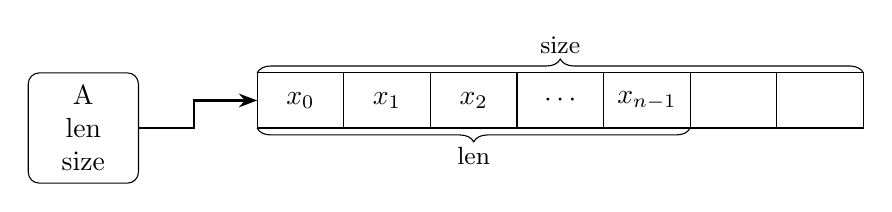
\begin{tikzpicture}[
  box/.style={draw, minimum width=1.4cm, minimum height=1.4cm, rounded corners}
]

% 尺寸与参数
\def\cellw{1.1cm}
\def\cellh{0.7cm}
\def\n{5}   % 已用长度 len
\def\m{7}   % 容量 size(m >= n)

% 左侧对象框 A/len/size
\node[box, align=center] (A) {A\\ len\\ size};

% 数组起点
\coordinate (S) at ($(A.east)+(1.5,0)$);

% 外框与分隔线
\draw (S) rectangle ++({\m*\cellw}, \cellh);
\foreach \i in {1,...,\numexpr\m-1\relax}
  \draw ($(S)+({\i*\cellw},0)$) -- ++(0,\cellh);

% 指针箭头
\draw[-{Stealth}, thick] (A.east) -- ++(0.7,0) |- ($(S)+(0,0.5*\cellh)$);

% 放几个标签
\node at ($(S)+({0.5*\cellw}, {0.5*\cellh})$) {$x_0$};
\node at ($(S)+({1.5*\cellw}, {0.5*\cellh})$) {$x_1$};
\node at ($(S)+({2.5*\cellw}, {0.5*\cellh})$) {$x_2$};
\node at ($(S)+({3.5*\cellw}, {0.5*\cellh})$) {$\cdots$};
\node at ($(S)+({(\n-1+0.5)*\cellw}, {0.5*\cellh})$) {$x_{n-1}$};

% 下面的大括号:len
\draw[decorate, decoration={brace, amplitude=5pt, mirror}]
  ($(S)+(0,0)$) -- ($(S)+({\n*\cellw},0)$)
  node[midway, yshift=-10pt, font=\small] {len};

% 上面的大括号:size
\draw[decorate, decoration={brace, amplitude=5pt}]
  ($(S)+(0,\cellh)$) -- ($(S)+({\m*\cellw},\cellh)$)
  node[midway, yshift=10pt, font=\small] {size};

\end{tikzpicture}

If want to do an insert\_last, just go to a of length and set it to x,
and increment length.

If len = size, we are going to allocate a new array, 
typically twice as big, and the resize operation takes $\theta(n)$ time ($\theta\left(\sum_{i=1}^{\log_{2} n} 2^i\right)$).

\section{amortization(摊还:把高昂操作的成本均摊到多次操作,分析平均复杂度)}
An operation takes $T(n)$ amortized time, if any $k$ operations takes $\leq k \cdot T(n)$ time.
(averaging over operation sequence)


Amortized analysis means spreading the cost of expensive operations over many cheap ones. 
For a dynamic array, most inserts take constant time $O(1)$, but sometimes the array is full and needs to resize, which costs $O(n)$. 
However, resizing does not happen every time---only occasionally (like doubling the size). 
If you insert $n$ items, the total cost of all resizes is about $2n$, so the average cost per insert is still $O(1)$. 
This is why we say appending to a dynamic array has amortized $O(1)$ time.




\begin{table}[h!]
\centering
\renewcommand{\arraystretch}{1.2}
\begin{tabular}{llcccccc}
\toprule
\multirow{2}{*}{Data Structure} & \multirow{2}{*}{Container} & 
\multicolumn{2}{c}{Static} & \multicolumn{4}{c}{Dynamic} \\
\cmidrule(lr){3-4} \cmidrule(lr){5-8}
& build($X$) & get\_at($i$) & set\_at($i,x$) & insert\_first($x$) & delete\_first() & insert\_last($x$) & delete\_last() \\
\midrule
Array & $O(n)$ & $O(1)$ & $O(1)$ & $O(n)$ & $O(n)$ & $O(1)$ & $O(1)$ \\
Linked List & $O(n)$ & $O(n)$ & $O(n)$ & $O(1)$ & $O(1)$ & $O(n)$ & $O(n)$ \\
Dynamic Array & $O(n)$ & $O(1)$ & $O(1)$ & $O(n)$ & $O(n)$ & $O(1)$ (amortized) & $O(1)$ (amortized) \\
\bottomrule
\end{tabular}
\caption{Worst-case and amortized time complexity of basic operations.}
\end{table}

\begin{table}[ht]
\centering
\begin{tabularx}{\textwidth}{|c|c|X|}
\hline
\textbf{Set 操作} & \textbf{含义} & \textbf{如何用 Sequence 实现} \\
\hline
insert(x)   & 插入元素 $x$(若已有相同 key 就替换) & 遍历 $seq[0..n-1]$,若有相同 key 则 set\_at(i, x),否则 insert\_last(x) \\
\hline
delete(k)   & 删除 $key=k$ 的元素 & 遍历 $seq[0..n-1]$,找到后执行 delete\_at(i) \\
\hline
find(k)     & 查找 $key=k$ 的元素 & 遍历 $seq[0..n-1]$,若 get\_at(i).key == k 则返回该元素 \\
\hline
find\_min() & 找到最小 key & 遍历所有元素,取最小 key \\
\hline
find\_max() & 找到最大 key & 遍历所有元素,取最大 key \\
\hline
find\_next(k) & 找到大于 k 的最小 key & 遍历所有元素,取所有 $x.key > k$ 的候选,返回最小的一个 \\
\hline
find\_prev(k) & 找到小于 k 的最大 key & 遍历所有元素,取所有 $x.key < k$ 的候选,返回最大的一个 \\
\hline
iter\_ord() & 按 key 顺序遍历 & 先调用 find\_min(),再不断调用 find\_next() \\
\hline
\end{tabularx}
\caption{Sequence 操作模拟 Set 操作的对照表}
\end{table}
%%----------- 参考文献 -------------------%%
%在reference.bib文件中填写参考文献,此处自动生成
\newpage
\reference


\end{document}